\chapter{Diarrheal Diseases}
\label{applications-short_dur}

Diarrheal diseases are a leading cause of childhood morbidity and mortality.  Defined as having loose or watery stools three or more times a day or more frequently than normal for the individual, the diarrheal episodes typically last 1-8 days for acute cases \cite{unicef_diarrhoea_2009, carlos_etiology_1990, lamberti_systematic_2012}.  Compared to many of the other diseases discussed thus far, diarrheal diseases have a very short duration.

Bacterial, viral and parasitic infections cause most cases of diarrhea.  Non-infectious causes include drugs, surgical conditions, systemic infections and food intolerance.  Typically spread via the oral-fecal route, water sanitation and hygiene is a large part of diarrhea prevention.  Treatment usually involves fluid replacement, as acute diarrhea causes fluid loss and dehydration.  Other common treatments are vitamin A and zinc supplementation, vaccinations and antibiotic regimes \cite{unicef_diarrhoea_2009, carlos_etiology_1990, lamberti_systematic_2012}.

For the analysis of diarrheal diseases, the primary sources of data are from surveys, hospital admissions and literature review.  The surveys report period prevalence data whereas hospital admissions and the majority of the literature report incidence data.  In short term diseases, point prevalence and incidence are approximately the same.  Therefore to avoid compositional bias, all incidence and period prevalence estimates were converted to point prevalence estimates using the assumption that
    \begin{equation}
    	p_{point}=i*d
    \end{equation}
where $p_{point}$ is the point prevalence, $i$ is the incidence and $d$ is the duration of the disease.  Thus the analysis includes 2029 rows of prevalence data from 19 regions.  Data from Central Latin America is shown in Figure \ref{fig:app-diarrhea data}.

    \begin{figure}[h]
        \begin{center}
            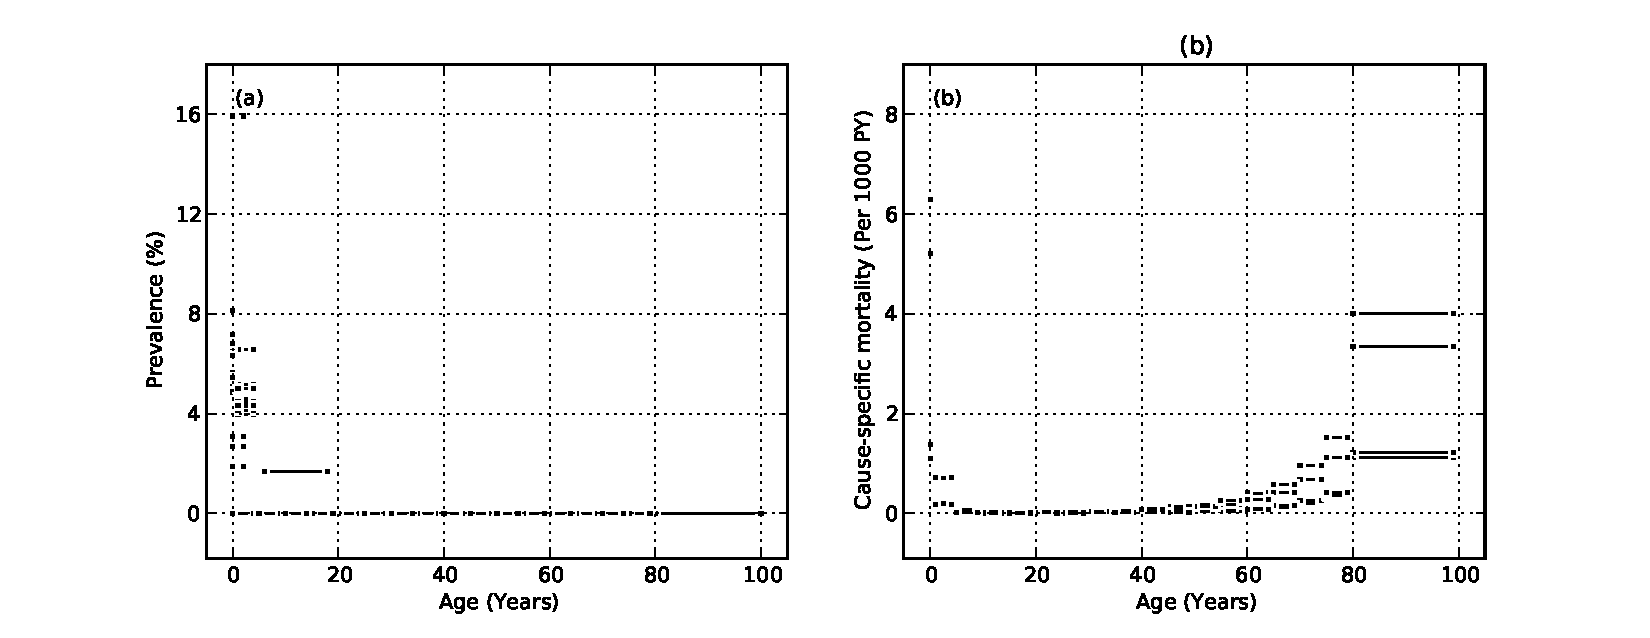
\includegraphics[width=\textwidth]{diarrhea-data.pdf}
            \caption{Diarrheal point prevalence (a) and cause-specific mortality (b) data in Central Latin America.}
            \label{fig:app-diarrhea data}
        \end{center}
    \end{figure}

Diarrheal diseases use a compartmental model to model all epidemiologic parameters for a single time, place and sex.  A compartmental model estimates all epidemiologic parameters simultaneously which maintains internally consistent results as discussed in Chapters \ref{sys-dynamics} and \ref{applications-fits_incon_v_con}.  In addition to the systematic review data, informative priors on the duration of diarrheal diseases help guide the modeling process.  The prior for duration is set as the prior for remission.  Duration priors produce less stable estimates than the more directly parameterized remission priors.  Therefore remission is the more appropriate prior for the model.  Equation \ref{eq:remission-duration} approximates the relationship between duration and remission
    \begin{equation} \label{eq:remission-duration}
    	r = \frac{1}{d}
    \end{equation}
where $r$ is the epidemiologic rate for remission and $d$ is the epidemiologic rate for duration in years.  Similar to the discussion of priors in Chapter \ref{applications-con_fit_splines}, the choice of priors affects the epidemiological estimates.  However, because of the logical requirement of internal consistency, a change in the duration of diarrheal diseases has effects on all epidemiological parameters as seen in Figure \ref{fig:app-diarrhea duration}.

    \begin{figure}[h]
        \begin{center}
            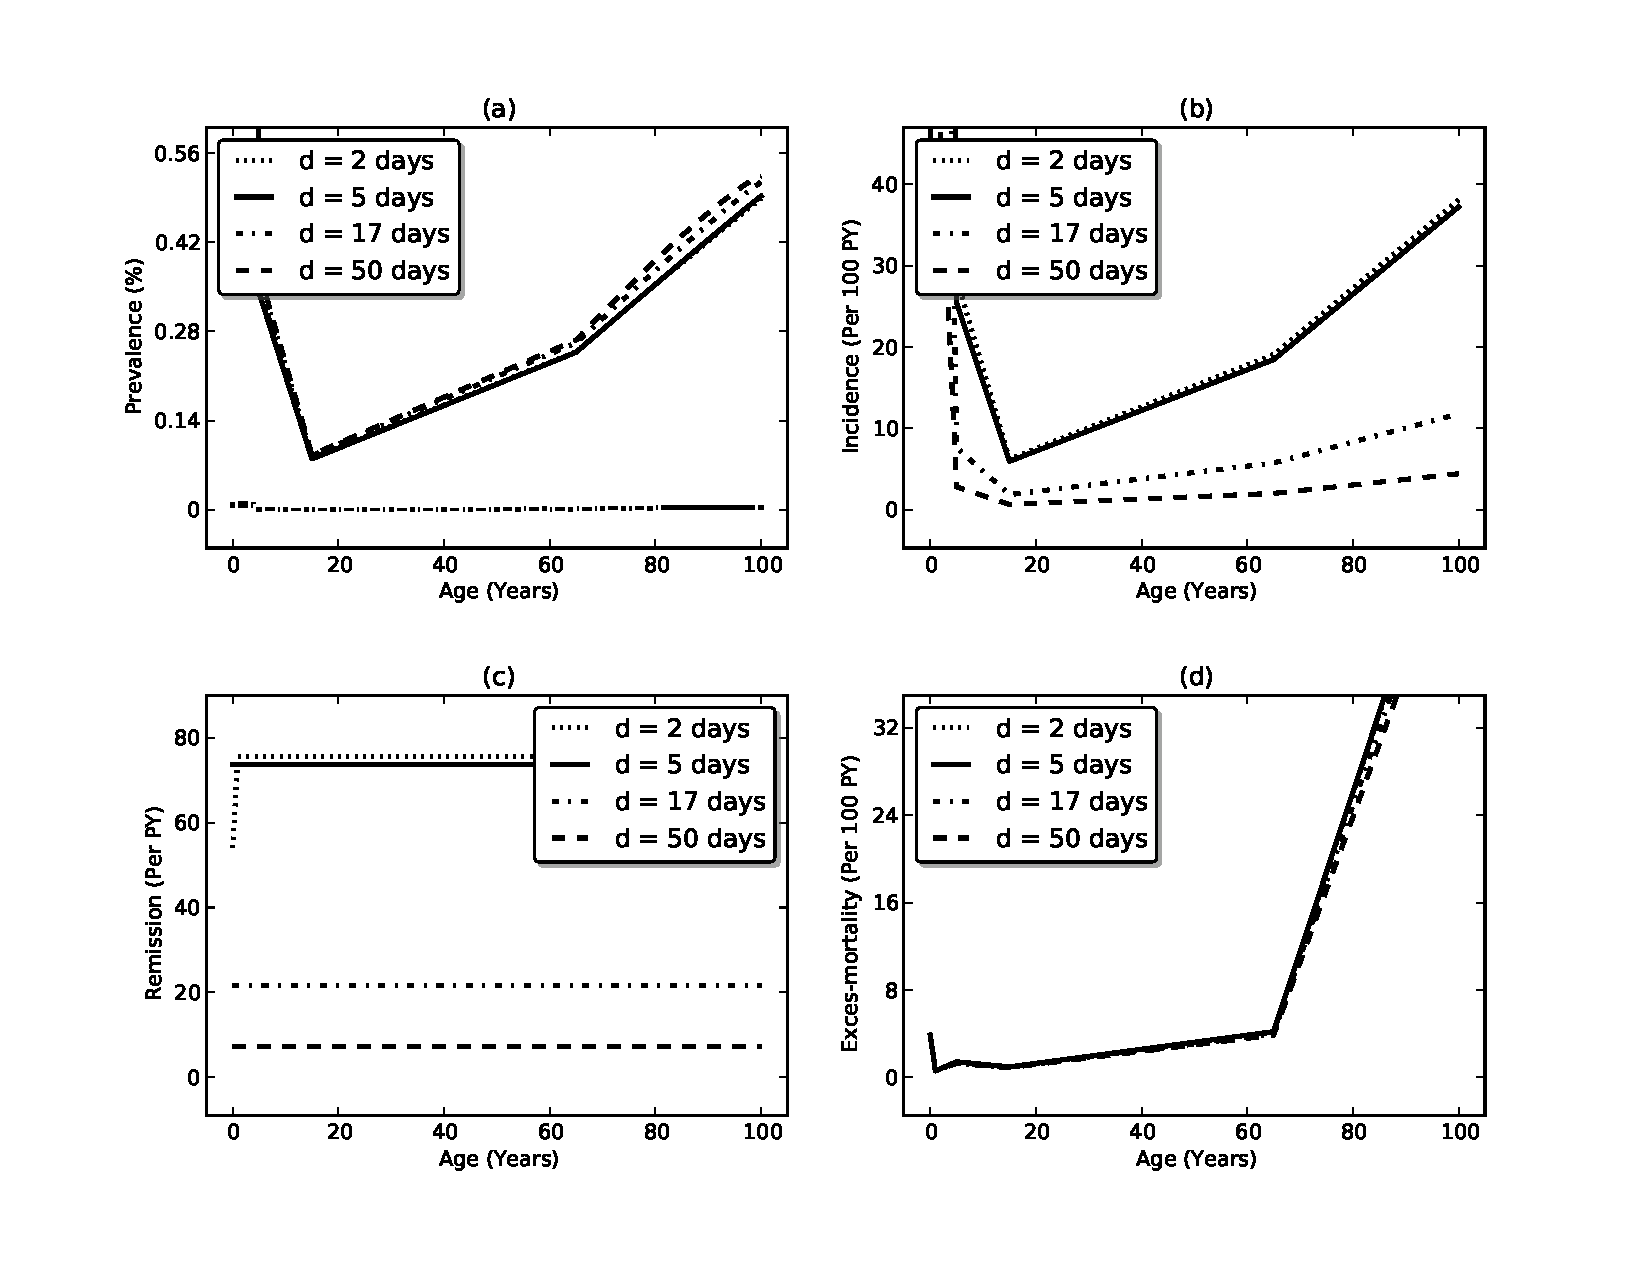
\includegraphics[width=\textwidth]{diarrhea-duration.pdf}
            \caption{Estimates of prevalence (a), incidence (b), remission (c) and excess-mortality (d) for diarrheal diseases in Central Latin American males in 2005 using a compartmental model.  The compartmental model requires internal consistency, so a change in the prior on duration has effects on all epidemiological parameters.}
            \label{fig:app-diarrhea duration}
        \end{center}
    \end{figure}
